
\documentclass[tikz, border=10pt]{standalone}
\usepackage{tikz}
\usetikzlibrary{positioning, chains, shapes.geometric, fit, shapes, arrows.meta, calc, backgrounds}

\begin{document}
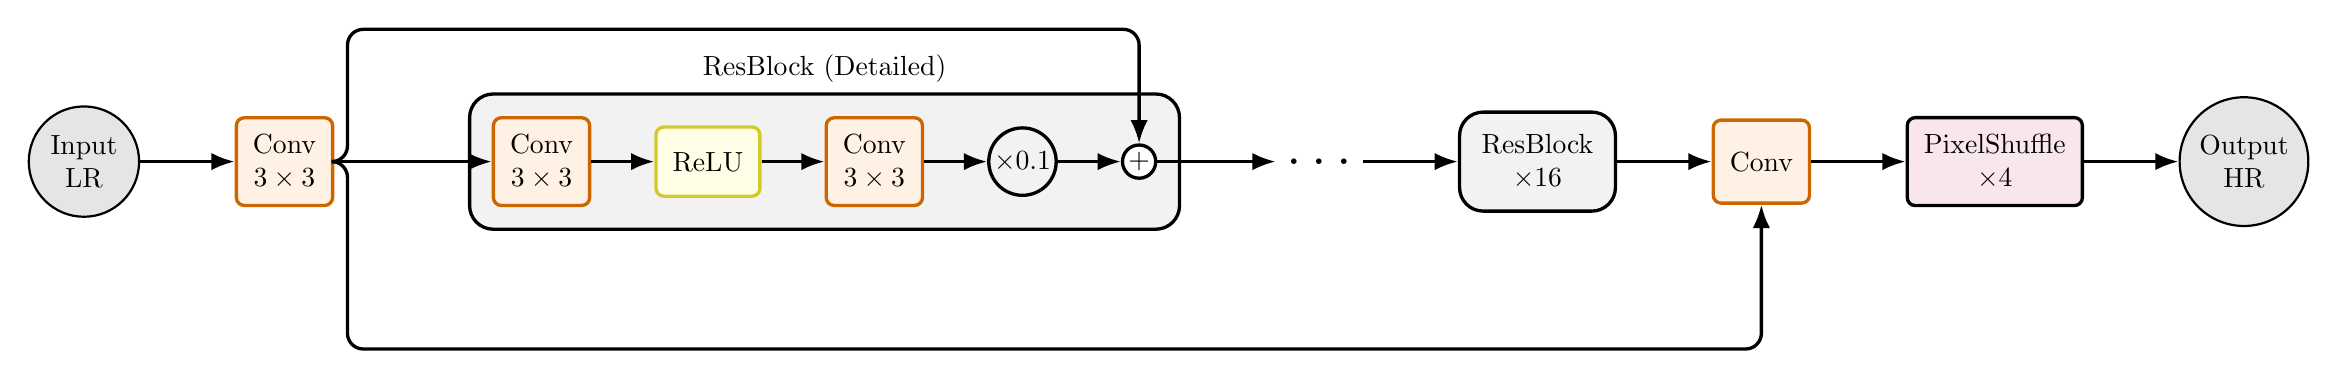
\begin{tikzpicture}[
    >=LaTeX, 
    very thick,
    node distance=1.0cm and 1.2cm,
    arrow/.style={
        ->,
        very thick,
        rounded corners=0.2cm
    },
    block/.style={
        rectangle,
        fill=gray!10,
        rounded corners=3mm,
        draw,
        very thick,
        inner sep=0.8em
    },
    layer/.style={
        rectangle,
        fill=white!10,
        rounded corners=1mm,
        inner xsep=0.6em,
        inner ysep=0.6em,
        minimum height=3.0em,
        align=center,
        draw,
        very thick
    },
    conv/.style={
        layer,
        fill=orange!10,
        draw=orange!80!black
    },
    relu/.style={
        layer,
        fill=yellow!10,
        draw=yellow!80!black,
        minimum height=2.5em
    },
    pool/.style={
        layer,
        fill=red!10,
        draw=red!80!black
    },
    input/.style={ 
        circle,
        minimum width=3.0em,
        draw,
        fill=gray!20,
        thick,
        align=center
    },
    sum/.style={
        circle,
        draw,
        fill=white,
        inner sep=0pt,
        minimum size=1.2em,
        node contents={+}
    }
]


    % Input
    \node[input] (in) {Input\\LR};

    % Head
    \node[conv, right=of in] (head) {Conv\\$3\times 3$};
    \draw[arrow] (in) -- (head);

    % ResBlock Detail
    \node[conv, right=2.0cm of head] (res1_c1) {Conv\\$3\times 3$};
    \node[relu, right=0.8cm of res1_c1] (res1_act) {ReLU};
    \node[conv, right=0.8cm of res1_act] (res1_c2) {Conv\\$3\times 3$};
    
    % Scaling constant
    \node[circle, draw, right=0.8cm of res1_c2, inner sep=1pt] (mul) {$\times 0.1$};
    
    % Sum
    \node (sum1) [sum, right=0.8cm of mul];

    % ResBlock Box
    \begin{scope}[on background layer]
        \node[block, fit=(res1_c1) (sum1), label=above:ResBlock (Detailed)] (resblock) {};
    \end{scope}

    % Connections inside ResBlock
    \draw[arrow] (head) -- (res1_c1);
    \draw[arrow] (res1_c1) -- (res1_act);
    \draw[arrow] (res1_act) -- (res1_c2);
    \draw[arrow] (res1_c2) -- (mul);
    \draw[arrow] (mul) -- (sum1);
    
    % Skip connection
    \draw[arrow] (head) -- ++(0.8,0) |- ($(resblock.north) + (0, 0.8)$) -| (sum1.north);

    % More Blocks (Abstract)
    \node[right=1.2cm of resblock] (dots) {\huge $\dots$};
    \draw[arrow] (sum1) -- (dots);

    \node[block, right=1.2cm of dots, minimum height=3em, align=center] (resN) {ResBlock\\$\times 16$};
    \draw[arrow] (dots) -- (resN);

    % Tail
    \node[conv, right=of resN] (tail) {Conv};
    \draw[arrow] (resN) -- (tail);

    % Global Skip
    \draw[arrow] (head) -- ++(0.8,0) |- ($(resblock.south) + (0, -1.5)$) -| (tail.south);

    % Upsampler
    \node[layer, right=of tail, fill=purple!10] (up) {PixelShuffle\\$\times 4$};
    \draw[arrow] (tail) -- (up);

    % Output
    \node[input, right=of up] (out) {Output\\HR};
    \draw[arrow] (up) -- (out);

\end{tikzpicture}
\end{document}
